\documentclass[conference]{IEEEtran}
\IEEEoverridecommandlockouts

\usepackage[utf8]{inputenc}
\usepackage[T1]{fontenc}
\usepackage[brazilian]{babel}
\usepackage{cite}
\usepackage{amsmath,amssymb,amsfonts}
\usepackage{graphicx}
\usepackage{textcomp}
\usepackage{xcolor}
\usepackage{booktabs}
\usepackage[locale=DE,group-separator={\,},group-minimum-digits=4]{siunitx}
\usepackage{url}

\newcommand{\repourl}{\url{https://github.com/lucthesloth/biometria26.2}}
\newcommand{\repoversion}{final-v1.0}
\newcommand{\BootN}{\num{10000}}
\newcommand{\TrainMin}{de 3,4 a 5,7}
\newcommand{\mapRegistros}{708}
\newcommand{\mapUnicos}{707}
\newcommand{\mapQualis}{438}
\newcommand{\mapTriagem}{269}
\newcommand{\mapTexto}{70}
\newcommand{\mapLidos}{70}
\newcommand{\mapIncl}{41}
\newcommand{\mapPend}{7}

\AtBeginDocument{\renewcommand{\IEEEkeywordsname}{Palavras-chave}}

\begin{document}

\title{Verificação 1:1 de impressões digitais com embeddings de CNN: ConvNeXt-Tiny, realce de cristas, transferência entre bases e fusão com minúcias}

\author{%
\IEEEauthorblockN{Lucas Ribeiro de Carvalho}
\IEEEauthorblockA{Universidade Tecnológica Federal do Paraná (UTFPR)\\
Ponta Grossa, Brasil\\
ORCID: \url{https://orcid.org/0009-0005-2339-0093}}
}

\maketitle

\begin{abstract}
Este trabalho avalia a verificação 1:1 de impressões digitais com embeddings de tamanho fixo gerados por CNNs pré-treinadas na ImageNet e ajustadas com poucas imagens. Ajustamos uma ConvNeXt-Tiny, uma ResNet-50 e uma EfficientNet-B0 com perda ArcFace em 480 imagens de 60 dedos da FVC2002 DB1, escolhemos a época e o limiar em 20 dedos de validação e testamos nos 30 dedos restantes. Sem novo ajuste, os mesmos modelos e limiares são avaliados na FVC2004 DB1, de outro sensor. A ConvNeXt-Tiny tem EER de 7,87\% na FVC2002 DB1 e de 8,32\% e 10,42\% na FVC2004 DB1, média de três seeds. Na base do treino, os intervalos de confiança por bootstrap não separam as três redes; na segunda base, a ConvNeXt-Tiny fica de 3,7 a 4,9 pontos abaixo das outras duas. O realce de cristas por filtros de Gabor não ajuda na base do treino e reduz a EER em 2,0 pontos nos 30 dedos de teste da FVC2004 DB1; no protocolo oficial o ganho não é conclusivo. O comparador de minúcias SourceAFIS tem EER de 2,71\% na FVC2002 DB1 e de 12,18\% no protocolo oficial da FVC2004 DB1, e a fusão dos dois scores chega a 2,73\% e 6,86\%. Um desfoque com $\sigma=3$ pixels leva a FMR da CNN a 76\%.
\end{abstract}

\begin{IEEEkeywords}
impressão digital, verificação biométrica, embedding de tamanho fixo, ArcFace, FVC2002, FVC2004, avaliação entre bases
\end{IEEEkeywords}

% ---------------------------------------------------------------------------
\section{Introdução}
\label{sec:intro}

Na verificação 1:1, o sistema recebe duas amostras e decide se elas vêm do mesmo dedo. Os comparadores clássicos de impressão digital extraem minúcias, isto é, terminações e bifurcações de cristas, e alinham dois conjuntos de tamanho variável a cada comparação~\cite{jain1997online,cappelli2010mcc,maltoni2022handbook}. Uma alternativa é treinar uma rede convolucional (CNN) que mapeia cada imagem para um vetor de tamanho fixo. A comparação passa a ser um produto interno entre dois vetores normalizados, e o template tem o mesmo tamanho para qualquer dedo~\cite{engelsma2021deepprint}.

Os modelos de tamanho fixo com resultados publicados nas bases FVC foram treinados com centenas de milhares de imagens. O DeepPrint usou \num{455000} impressões roladas de \num{38291} dedos~\cite{engelsma2021deepprint}, e o AFR-Net usou cerca de 1,3 milhão de imagens~\cite{grosz2024afrnet}. Este trabalho pergunta o que uma CNN pré-treinada na ImageNet~\cite{deng2009imagenet} consegue quando o ajuste fino dispõe de 480 imagens de um único sensor, quanto desse desempenho sobrevive à troca de sensor e o que o embedding acrescenta a um comparador de minúcias.

O estudo segue a ficha da disciplina: a base principal é a FVC2002 DB1, a segunda é a FVC2004 DB1~\cite{maio2002fvc2002,maio2004fvc2004}, e as duas entram com os conjuntos A e B (110 dedos cada). Há quatro experimentos: a base principal (A); três CNNs nas duas bases (B); a segunda base com modelo e limiar congelados (C); e a robustez a desfoque e rotação (D). As contribuições são duas. A primeira é o protocolo, em que a época e o limiar saem de dedos de validação e são reutilizados sem mudança no teste e na segunda base. A segunda é a comparação de três CNNs, com três seeds e intervalos de confiança pareados. Os mesmos pares avaliam um comparador de minúcias, a fusão com ele, a rede sem ajuste fino e a ablação do realce de cristas. Código, protocolos e scores estão em \repourl, versão \texttt{\repoversion}.

% ---------------------------------------------------------------------------
\section{Trabalhos relacionados}
\label{sec:relacionados}
Esta seção resume um mapeamento sistemático feito segundo Kitchenham e Charters~\cite{kitchenham2007guidelines}, com a etapa de classificação de Petersen et~al.~\cite{petersen2015guidelines}. Ele tem seis questões: arquitetura e perda (QP1), tipo de representação e comparação (QP2), bases e protocolo (QP3), métricas de desempenho e de custo (QP4), avaliação entre bases e robustez (QP5) e pré-processamento com ablação (QP6).

\subsection{Método}

A busca foi feita no OpenAlex, com a string aplicada a título e resumo, de 2015 a 2026. Ela trouxe \mapRegistros{} registros, \mapUnicos{} sem duplicatas. Ficaram só periódicos Qualis A1 a A4 da área Computação (lista 2017-2020), o que excluiu \mapQualis{} registros e deixou \mapTriagem{} para triagem. Entram estudos primários de impressão digital em que uma rede convolucional gera a representação ou o score de comparação e que reportam desempenho de comparação; estudos que medem só acurácia de classificação ficam fora. Cada decisão foi registrada com critério e justificativa. Uma segunda triagem às cegas de 54 registros (20\%) deu kappa de Cohen de 0,873 (três classes). A triagem enviou \mapTexto{} estudos à leitura completa. O snowballing para trás~\cite{wohlin2014snowballing} achou 13 registros novos: 7 seguiram para a leitura e 6 foram excluídos, 3 deles porque não existem (referências fabricadas por um dos estudos incluídos, com DOIs de outros artigos). Dos 77 estudos enviados à leitura, lemos \mapLidos{}, 11 na versão arXiv, e incluímos \mapIncl{}; os outros \mapPend{} não foram obtidos.

\subsection{Resultados por questão}

\emph{QP1 e QP2.} Vinte dos \mapIncl{} estudos usam arquitetura própria, 9 usam transformadores ou redes híbridas, entre eles~\cite{qiu2024ifvit,grosz2024afrnet,guan2024jipnet}, e 5 usam ResNet. Três declaram pré-treino na ImageNet, e 3 usam perda de margem angular do tipo ArcFace ou CosFace, entre eles o AFR-Net~\cite{grosz2024afrnet}. Vinte e dois produzem um vetor de tamanho fixo, como o DeepPrint~\cite{engelsma2021deepprint}, de 192 dimensões, e 8 geram o score direto por rede siamesa.

\emph{QP3 e QP4.} A FVC2004 aparece em 14 estudos e a FVC2002 em 13, mas só 9 seguem o protocolo oficial FVC, entre eles~\cite{engelsma2021deepprint,qiu2024ifvit,grosz2024afrnet}; nele, o DeepPrint chega a TAR de 97,5\% a FAR de 0,1\% na FVC2004 DB1-A. A divisão disjunta por identidade é relatada em 25, 12 não a descrevem e 4 não a usam. Só 6 escolhem limiar ou hiperparâmetros sem usar o teste, e outros 14 o fazem em parte. A EER aparece em 26 estudos e FMR/FNMR em 13; o custo aparece sobretudo como tempo (29).

\emph{QP5 e QP6.} Vinte e quatro estudos avaliam entre bases, por exemplo treinando com impressões sintéticas~\cite{engelsma2022printsgan} ou com uma base própria e testando em FVC e NIST~\cite{liu2019aligned}. Vinte e cinco não testam robustez; os outros 16 testam sobretudo captura parcial (9) e rotação (4)~\cite{guan2024jipnet}, e só um mede desfoque, por EER e AUC, sem limiar fixo. Onze estudos fazem ablação de etapas do pipeline. Código ou modelos estão disponíveis em 5 estudos.

\subsection{Lacuna e ameaças à validade}

Entre os \mapIncl{} estudos, só um mede desfoque, sem limiar fixo, e só 6 escolhem limiar ou hiperparâmetros sem usar o teste. Este trabalho fixa o limiar em dedos de validação, reaplica-o sem mudança ao teste e a uma segunda base de outro sensor, e mede desfoque e rotação em quatro níveis.

O mapeamento tem um único revisor, e a segunda triagem às cegas não substitui um segundo. A lista Qualis deixa fora conferências como IJCB, ICB e CVPR, a busca usou só o OpenAlex, e \mapPend{} textos não foram lidos; as contagens são um retrato parcial da literatura.


% ---------------------------------------------------------------------------
\section{Base de dados}
\label{sec:dados}

\subsection{Bases}

As bases FVC2002 DB1 e FVC2004 DB1 vêm das competições de verificação do BioLab da Universidade de Bolonha~\cite{maio2002fvc2002,maio2004fvc2004}. A FVC2002 DB1 usa o sensor óptico Identix TouchView~II ($388\times374$ pixels, 500~dpi) e a FVC2004 DB1 o óptico CrossMatch V300 ($640\times480$ pixels, 500~dpi); a coleta da FVC2004 pediu de propósito variações de pressão, rotação e umidade~\cite{maio2004fvc2004}. Cada base tem o conjunto A, com 100 dedos, e o conjunto B, com 10 dedos (101 a 110), sempre com 8 impressões por dedo: \num{880} imagens por base. Os dois conjuntos estão no material suplementar do capítulo~4 do \emph{Handbook of Fingerprint Recognition}~\cite{maltoni2022handbook}.

\subsection{Divisão por identidade}

Com seed 42, os 110 dedos da FVC2002 DB1 são divididos em 60 para treino (480 imagens), 20 para validação (160) e 30 para teste (240), sem que um dedo apareça em mais de uma parte (Tabela~\ref{tab:bases}). A validação escolhe a época e fixa o limiar; o teste dá o Experimento~A. A FVC2004 DB1 nunca entra no treino. A mesma função e a mesma seed geram a divisão dela, e seus 30 dedos de teste dão o Experimento~C. Na FVC2004 DB1 avaliamos também o protocolo oficial da competição no conjunto A inteiro. Não usamos o protocolo oficial da FVC2002 DB1 porque 72 dos 100 dedos do seu conjunto A estão no treino ou na validação.

\begin{table}[t]
\centering
\caption{Bases e divisão por identidade (seed 42). Dedos$\times$impressões.}
\label{tab:bases}
\footnotesize
\setlength{\tabcolsep}{3pt}
\begin{tabular}{@{}lccc@{}}
\toprule
Base & Treino & Validação & Teste \\
\midrule
FVC2002 DB1 (A+B) & $60\times8$ & $20\times8$ & $30\times8$ (Exp.~A) \\
FVC2004 DB1 (A+B) & -- & -- & $30\times8$ (Exp.~C) \\
FVC2004 DB1-A, oficial & -- & -- & $100\times8$ (Exp.~C) \\
\bottomrule
\end{tabular}
\end{table}

\subsection{Pares de comparação}

Os pares genuínos são todas as combinações de duas impressões do mesmo dedo, $\binom{8}{2}=28$ por dedo, e os impostores são todos os pares de imagens de dedos diferentes. A validação tem 560 genuínos e \num{12160} impostores; cada conjunto de teste de 30 dedos tem 840 genuínos e \num{27840} impostores. O protocolo oficial compara, no conjunto A, todas as impressões do mesmo dedo (\num{2800} genuínos) e a primeira impressão de cada dedo com a primeira dos outros (\num{4950} impostores)~\cite{maio2004fvc2004}. As três CNNs e as referências usam os mesmos arquivos \texttt{protocols/*/test\_pairs.csv}.

% ---------------------------------------------------------------------------
\section{Metodologia}
\label{sec:metodologia}

\begin{figure*}[t]
\centering
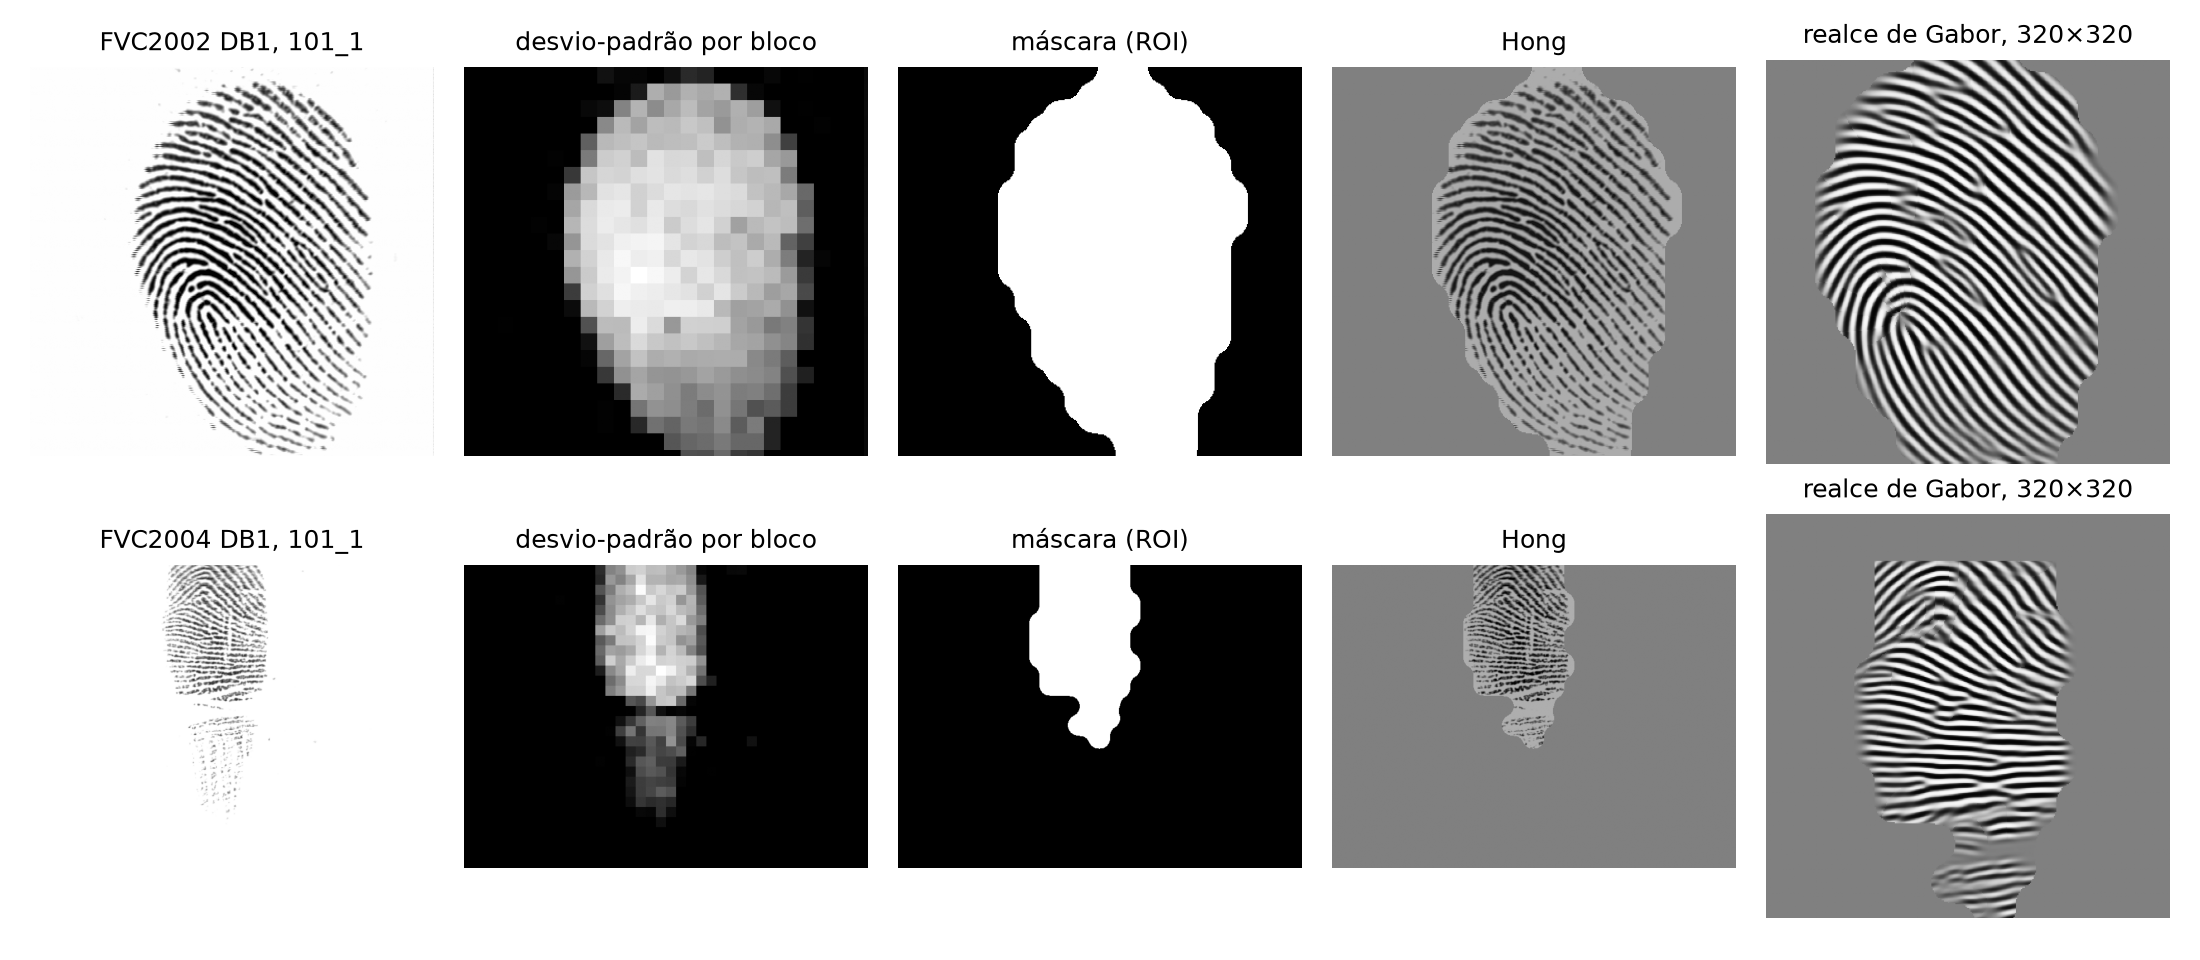
\includegraphics[width=0.7\textwidth]{figures/pipeline.png}
\caption{Etapas do pré-processamento para uma imagem da FVC2002 DB1-B (acima) e uma da FVC2004 DB1-B (abaixo): imagem bruta, mapa de desvio-padrão por bloco, máscara da ROI, imagem após a normalização de Hong e entrada da rede, com realce de Gabor, de $320\times320$ pixels.}
\label{fig:pipeline}
\end{figure*}

As três CNNs recebem o mesmo pré-processamento, e todos os parâmetros ficam em \texttt{config.yaml}.

\subsection{Pré-processamento}

A Fig.~\ref{fig:pipeline} mostra as etapas em duas imagens reais. O pipeline padrão do enunciado é ROI, tons de cinza, normalização e redimensionamento. Desviamos dele em dois pontos. Acrescentamos o realce de cristas, que teve a menor EER de validação na fase anterior do projeto e cuja ablação está na Seção~\ref{sec:resultados}. E trocamos o redimensionamento por uma janela fixa, para que a distância entre cristas chegue à rede na mesma escala nos dois sensores.

\emph{Reamostragem.} Toda imagem vai a 500~dpi antes das outras etapas, para que a janela fixa cubra a mesma área física em qualquer sensor; nas duas bases deste trabalho a resolução nativa já é 500~dpi.

\emph{Segmentação da ROI.} Calculamos o desvio-padrão de intensidade em blocos de $16\times16$ pixels, cerca de dois períodos de crista a 500~dpi, seguindo a segmentação por estatísticas de bloco descrita em~\cite{maltoni2022handbook}. O limiar de Otsu~\cite{otsu1979threshold} separa os blocos de impressão do fundo. Em seguida aplicamos fechamento e abertura morfológicos com um elemento elíptico de $33\times33$ pixels, mantemos o maior componente conexo e preenchemos os buracos.

\emph{Controle de qualidade.} Uma amostra conta como falha de aquisição (FTA) quando a área da ROI é menor que 40~mm$^2$, cerca de \num{15500} pixels a 500~dpi. A regra foi fixada antes do primeiro treino, portanto antes de qualquer score de teste. A FTA ficou em 0\% nas \num{1760} imagens das duas bases. A Seção~\ref{sec:protocolo} diz o que acontece com os pares de uma amostra em FTA.

\emph{Normalização.} A imagem em tons de cinza passa pela normalização de Hong, Wan e Jain~\cite{hong1998enhancement}, que leva a média e a variância dentro da ROI a $M_0=128$ e $V_0=2500$ (desvio-padrão 50), com o resultado truncado em $[0,255]$. Fora da ROI, o valor é 128.

\emph{Realce de cristas.} Sobre a imagem normalizada aplicamos a filtragem contextual de Hong, Wan e Jain~\cite{hong1998enhancement}, simplificada: um período de crista por imagem, tirado do pico do espectro de potência radial entre 5 e 15 pixels, e um banco de 16 filtros de Gabor, escolhidos em cada pixel pela orientação local do tensor de estrutura. A resposta passa por uma tangente hiperbólica e volta a $[0,255]$. O objetivo do filtro é manter a geometria das cristas e reduzir as diferenças de contraste e textura entre sensores (Fig.~\ref{fig:pipeline}). O realce custou de 76 a 125~ms por imagem em CPU, contra 20 a 30~ms do pipeline sem ele.

\emph{Janela fixa.} Recortamos $320\times320$ pixels centrados no centroide da ROI, completando com 128 além da borda, sem redimensionar cada imagem, para que a distância entre cristas fique igual entre sensores. A rede recebe os níveis de cinza em $[-1,1]$.

\subsection{Arquitetura}

As três redes vêm da torchvision~\cite{paszke2019pytorch}, pré-treinadas na ImageNet-1k~\cite{deng2009imagenet}. A primeira convolução recebe um canal, com os pesos somados sobre RGB. A camada de classificação dá lugar a Dropout de 0,2, uma camada linear para 256 dimensões e BatchNorm1d, e a saída normalizada em L2 é o template. A rede principal é a ConvNeXt-Tiny~\cite{liu2022convnext} (\texttt{IMAGENET1K\_V1}): mantemos a LayerNorm que segue o \emph{pooling} global, congelamos \texttt{features.0} a \texttt{features.3} (entrada e os dois primeiros estágios) e treinamos os estágios 3 e 4; são 28,01~M parâmetros, 26,78~M treináveis. As outras duas servem de comparação: a ResNet-50~\cite{he2016resnet} (\texttt{IMAGENET1K\_V2}), com \texttt{conv1}, \texttt{bn1}, \texttt{layer1} e \texttt{layer2} congeladas e as BatchNorm congeladas em modo de avaliação, 24,03~M parâmetros e 22,59~M treináveis; e a EfficientNet-B0~\cite{tan2019efficientnet} (\texttt{IMAGENET1K\_V1}), congelada até \texttt{features.3}, com 4,34~M parâmetros, 4,27~M treináveis. Nas três redes, os blocos congelados vão até o fim do segundo estágio.

\subsection{Treino}

Durante o treino, uma cabeça ArcFace~\cite{deng2019arcface} recebe o embedding $\mathbf{e}$ e os pesos normalizados das 60 identidades de treino. Para a classe correta $y$, o logit é $s\cos(\theta_y+m)$; para as demais, $s\cos\theta_j$, em que $\theta_j$ é o ângulo entre $\mathbf{e}$ e o peso da classe $j$. A perda é a entropia cruzada sobre esses logits, com $m=0{,}3$ e $s=30$, e a cabeça é descartada depois do treino.

Cada lote tem 16 identidades com 4 impressões (esquema P$\times$K~\cite{hermans2017triplet}). Usamos AdamW~\cite{loshchilov2019adamw} com taxa de $3\times10^{-4}$, decaimento de pesos $5\times10^{-4}$, decaimento cosseno em 80 épocas e bfloat16 na GPU. O aumento de dados aplica rotação de até $30^\circ$, translação de até 10\%, desfoque gaussiano (probabilidade 0,3, $\sigma$ de 0,1 a 1,5) e variação de brilho e contraste de 0,2, sem espelhamento nem zoom. Guardamos o modelo da época com menor EER na validação.

Essa configuração vem de uma fase anterior do projeto, sem o conjunto A, em que a rede foi ajustada no conjunto B de outras bases FVC e validada em sensores fora do treino; lá, o realce de Gabor e as 80 épocas tiveram a menor EER de validação entre seis candidatas. A configuração foi congelada antes destes treinos, e as três redes usam a mesma. Dois dedos do teste atual já estavam no teste daquela fase; a Seção~\ref{sec:discussao} mede o efeito disso.

O score é a similaridade de cosseno $s=\mathbf{e}_a^\top\mathbf{e}_b$, e o par é aceito quando $s\ge t$. O limiar $t$ é o da EER nos pares de validação, fixado uma vez por modelo e seed e reutilizado sem mudança em todos os testes e níveis de degradação.

% ---------------------------------------------------------------------------
\section{Protocolo experimental}
\label{sec:protocolo}

\subsection{Divisões, pares e seeds}

Treino, validação e teste não compartilham dedos (Tabela~\ref{tab:bases}); a divisão e os pares usam a seed 42. Cada modelo é treinado com as seeds 2026, 1999 e 1234, e reportamos média e desvio-padrão amostral, uma estimativa grosseira com três execuções. Como a validação escolhe a época e o limiar, sua EER é otimista.

\subsection{Limiar e métricas}

Para um limiar $t$, a FMR é a fração de pares impostores com $s\ge t$ e a FNMR é a fração de pares genuínos com $s<t$. Reportamos as duas no limiar $t$ congelado. A EER de cada teste, interpolada entre os dois limiares em que FNMR$-$FMR muda de sinal, só compara a separação das classes. Testes unitários conferem EER e AUC contra o scikit-learn. Também mostramos a TAR a FAR de 1\%, a ROC e as distribuições de scores. Os intervalos de confiança de 95\% vêm de um bootstrap sobre dedos (\texttt{scripts/bootstrap\_ci.py}), com \BootN{} reamostragens dos 30 dedos de cada teste (100 no protocolo oficial): um dedo sorteado $m$ vezes entra $m$ vezes com seus pares genuínos, e seus pares impostores entram na proporção do produto das multiplicidades. Cada réplica usa os mesmos dedos para todos os modelos e seeds, o que torna pareadas as diferenças de EER. Os intervalos medem a incerteza da amostra de dedos para as três seeds treinadas e não incluem a variação entre treinos. Nos Experimentos A, B e C, um par com uma amostra em FTA sairia do cálculo de FMR e FNMR, com a FTA reportada à parte~\cite{iso19795-1}; não houve nenhuma FTA nessas imagens.

\subsection{Experimentos}

\emph{A.} As três CNNs nos 30 dedos de teste da FVC2002 DB1. \emph{B.} As mesmas redes nas duas bases, nos mesmos pares. O enunciado prevê cruzar as CNNs de duas equipes; sem os scores da outra equipe, o experimento compara as nossas três redes, e \texttt{scripts/import\_scores.py} aceita os scores dela nos mesmos pares. \emph{C.} Os mesmos modelos e limiares, sem novo ajuste, na FVC2004 DB1: nos 30 dedos de teste e no protocolo oficial do conjunto A. \emph{D.} Nas imagens brutas dos 30 dedos de teste da FVC2002 DB1, degradamos as duas imagens de cada par e repetimos o pipeline com a ConvNeXt-Tiny e o limiar congelados: desfoque gaussiano com $\sigma\in\{0,1,2,3\}$ pixels e rotação de $\{0^\circ,10^\circ,20^\circ,30^\circ\}$, com sinal sorteado por imagem (seed fixa) e fundo na mediana da imagem. Só neste experimento mantemos os pares com amostra em FTA e reportamos a FTA de cada nível à parte, porque descartá-los tiraria da conta as capturas mais degradadas. \emph{Ablação.} A ConvNeXt-Tiny sem o realce de Gabor (só a normalização de Hong), com as mesmas épocas, seeds e protocolos. \emph{Referências.} O SourceAFIS 3.18.1~\cite{vazan2024sourceafis}, um comparador de minúcias de código aberto, recebe as imagens brutas, usa os parâmetros padrão e os mesmos pares, e seu limiar também é o da EER na validação. Na fusão, o score de cada comparador é normalizado pela média e pelo desvio-padrão dos seus impostores de validação, e o score final é $w\,z_{\text{CNN}}+(1-w)\,z_{\text{min}}$; o peso $w$, numa grade de 0,1, e o limiar vêm da EER na validação (\texttt{scripts/fusion.py}). A última referência é a ConvNeXt-Tiny da ImageNet sem ajuste fino: o vetor de 768 dimensões que sai do \emph{pooling} global e da LayerNorm, normalizado em L2, nas imagens com realce.

\subsection{Hardware, software e custo}

Usamos um AMD Ryzen~5 5600X, 32~GB de RAM e uma NVIDIA GeForce RTX~4060 de 8~GB, com Windows~11, Python 3.13 e PyTorch 2.6.0 (CUDA 12.4). Um treino leva \TrainMin{} minutos. A latência é medida só na rede, com lote de uma imagem de $320\times320$, 20 passagens de aquecimento e 100 repetições sincronizadas com a GPU. O texto usa a mediana; a média está na Tabela~\ref{tab:padrao}.

% ---------------------------------------------------------------------------
\section{Resultados}
\label{sec:resultados}

Os valores são média $\pm$ desvio-padrão amostral sobre as seeds 2026, 1999 e 1234 (\texttt{results/summary.md}), e os intervalos estão em \texttt{results/bootstrap\_ci.csv}.

\begin{table*}[t]
\centering
\caption{Experimentos A, B e C, ablação e referências: todos os pares nos testes de 30 dedos e protocolo oficial na FVC2004 DB1-A. CNX s/ realce: ConvNeXt-Tiny só com a normalização de Hong. CNX s/ ajuste: ConvNeXt-Tiny da ImageNet sem ajuste fino. SourceAFIS: comparador de minúcias. Fusão: ConvNeXt-Tiny com SourceAFIS. As linhas com $\pm$ são média e desvio-padrão de três seeds; as demais têm uma execução. IC 95\%: bootstrap sobre dedos, da EER média. FMR e FNMR no limiar congelado da validação. Taxas em \%.}
\label{tab:expB}
\footnotesize
\setlength{\tabcolsep}{4pt}
\begin{tabular}{@{}llcccccc@{}}
\toprule
Avaliação (gen./imp.) & Modelo & EER & IC 95\% da EER & AUC & FMR & FNMR & TAR@FAR=1\% \\
\midrule
Teste, FVC2002 DB1 & ConvNeXt-Tiny & $7{,}87\pm0{,}29$ & 5,6 a 10,0 & $0{,}9762\pm0{,}0012$ & $6{,}39\pm1{,}02$ & $9{,}56\pm1{,}34$ & $68{,}81\pm2{,}38$ \\
(30 dedos, exp. A) & ResNet-50 & $9{,}54\pm0{,}95$ & 7,2 a 11,7 & $0{,}9681\pm0{,}0051$ & $7{,}58\pm1{,}05$ & $11{,}63\pm2{,}82$ & $65{,}79\pm2{,}95$ \\
(840/\num{27840}) & EfficientNet-B0 & $7{,}92\pm0{,}40$ & 5,8 a 10,1 & $0{,}9777\pm0{,}0011$ & $7{,}12\pm0{,}81$ & $8{,}69\pm1{,}31$ & $71{,}15\pm4{,}01$ \\
 & CNX s/ realce & $6{,}89\pm0{,}78$ & 5,2 a 8,3 & $0{,}9830\pm0{,}0009$ & $8{,}36\pm0{,}63$ & $5{,}48\pm0{,}94$ & $74{,}44\pm2{,}02$ \\
 & CNX s/ ajuste & 29,49 & 26,7 a 32,5 & 0,7760 & 40,72 & 23,10 & 24,64 \\
 & SourceAFIS & 2,71 & 1,4 a 4,0 & 0,9887 & 3,83 & 2,38 & 96,31 \\
 & Fusão & $2{,}73\pm0{,}11$ & 1,1 a 4,4 & $0{,}9934\pm0{,}0001$ & $3{,}27\pm0{,}64$ & $2{,}66\pm0{,}25$ & $96{,}87\pm0{,}25$ \\
\midrule
Teste, FVC2004 DB1 & ConvNeXt-Tiny & $8{,}32\pm0{,}44$ & 6,3 a 11,0 & $0{,}9659\pm0{,}0026$ & $6{,}92\pm1{,}06$ & $10{,}79\pm2{,}65$ & $46{,}47\pm2{,}15$ \\
(30 dedos, exp. C) & ResNet-50 & $13{,}20\pm0{,}64$ & 10,4 a 16,0 & $0{,}9367\pm0{,}0027$ & $8{,}53\pm1{,}50$ & $19{,}29\pm2{,}03$ & $36{,}31\pm2{,}84$ \\
(840/\num{27840}) & EfficientNet-B0 & $12{,}24\pm0{,}39$ & 9,8 a 14,8 & $0{,}9461\pm0{,}0031$ & $7{,}44\pm1{,}31$ & $19{,}09\pm2{,}16$ & $46{,}19\pm3{,}09$ \\
 & CNX s/ realce & $10{,}35\pm0{,}72$ & 8,5 a 12,5 & $0{,}9553\pm0{,}0058$ & $11{,}22\pm1{,}00$ & $9{,}29\pm0{,}78$ & $38{,}10\pm4{,}88$ \\
 & CNX s/ ajuste & 34,88 & 31,8 a 37,8 & 0,7131 & 18,68 & 52,74 & 10,60 \\
 & SourceAFIS & 9,31 & 6,6 a 12,4 & 0,9554 & 2,02 & 12,62 & 85,00 \\
 & Fusão & $4{,}96\pm0{,}25$ & 3,3 a 6,9 & $0{,}9881\pm0{,}0012$ & $3{,}08\pm0{,}74$ & $7{,}34\pm1{,}92$ & $87{,}78\pm0{,}61$ \\
\midrule
FVC2004 DB1-A, & ConvNeXt-Tiny & $10{,}42\pm0{,}17$ & 9,1 a 11,9 & $0{,}9553\pm0{,}0016$ & $7{,}57\pm1{,}07$ & $14{,}10\pm1{,}70$ & $50{,}89\pm2{,}65$ \\
protocolo oficial & ResNet-50 & $14{,}78\pm1{,}02$ & 13,2 a 16,4 & $0{,}9240\pm0{,}0078$ & $9{,}64\pm1{,}62$ & $21{,}65\pm1{,}92$ & $33{,}00\pm4{,}12$ \\
(\num{2800}/\num{4950}) & EfficientNet-B0 & $14{,}08\pm0{,}46$ & 12,7 a 15,7 & $0{,}9320\pm0{,}0020$ & $9{,}21\pm0{,}94$ & $20{,}82\pm1{,}61$ & $39{,}82\pm2{,}35$ \\
 & CNX s/ realce & $11{,}29\pm0{,}84$ & 9,9 a 12,9 & $0{,}9484\pm0{,}0087$ & $11{,}45\pm1{,}01$ & $11{,}21\pm0{,}81$ & $32{,}74\pm7{,}07$ \\
 & CNX s/ ajuste & 34,75 & 31,8 a 37,8 & 0,7157 & 19,49 & 50,25 & 11,25 \\
 & SourceAFIS & 12,18 & 10,4 a 14,4 & 0,9350 & 4,59 & 15,82 & 79,14 \\
 & Fusão & $6{,}86\pm0{,}41$ & 5,6 a 8,1 & $0{,}9801\pm0{,}0019$ & $3{,}62\pm0{,}83$ & $10{,}04\pm1{,}95$ & $83{,}11\pm0{,}62$ \\
\bottomrule
\end{tabular}
\end{table*}

\begin{table}[t]
\centering
\caption{Ficha do sistema com a ConvNeXt-Tiny, nos 30 dedos de teste de cada base. Taxas em \%.}
\label{tab:padrao}
\footnotesize
\setlength{\tabcolsep}{3pt}
\begin{tabular}{@{}lcc@{}}
\toprule
Informação & FVC2002 DB1 & FVC2004 DB1 \\
 & (principal) & (entre bases) \\
\midrule
Modalidade, CNN & \multicolumn{2}{c}{impressão digital 1:1, ConvNeXt-Tiny} \\
Pesos, ajuste & \multicolumn{2}{c}{ImageNet-1k (V1); ArcFace, 60 dedos FVC2002} \\
Parâmetros & \multicolumn{2}{c}{28,01~M (26,78~M treináveis)} \\
Embedding & \multicolumn{2}{c}{256 dimensões, norma L2} \\
Comparação & \multicolumn{2}{c}{similaridade de cosseno} \\
Limiar & \multicolumn{2}{c}{$0{,}368\pm0{,}010$ (EER na validação)} \\
\midrule
EER & $7{,}87\pm0{,}29$ & $8{,}32\pm0{,}44$ \\
AUC & $0{,}9762\pm0{,}0012$ & $0{,}9659\pm0{,}0026$ \\
FMR & $6{,}39\pm1{,}02$ & $6{,}92\pm1{,}06$ \\
FNMR & $9{,}56\pm1{,}34$ & $10{,}79\pm2{,}65$ \\
TAR@FAR=1\% & $68{,}81\pm2{,}38$ & $46{,}47\pm2{,}15$ \\
FTA & 0,00 & 0,00 \\
\midrule
Inferência & \multicolumn{2}{c}{média 9,67~ms, mediana 8,87~ms (lote 1)} \\
Tamanho & \multicolumn{2}{c}{112,1~MB (\texttt{state\_dict})} \\
Hardware & \multicolumn{2}{c}{RTX~4060 8~GB, Ryzen~5 5600X, 32~GB de RAM} \\
\bottomrule
\end{tabular}
\end{table}

\begin{table}[t]
\centering
\caption{Custo das três CNNs: rede isolada, lote de uma imagem de $320\times320$ na RTX~4060.}
\label{tab:custo}
\footnotesize
\setlength{\tabcolsep}{3pt}
\begin{tabular}{@{}lcccc@{}}
\toprule
Rede & Parâmetros & Pesos & Mediana & Média \\
 & (M) & (MB) & (ms) & (ms) \\
\midrule
ConvNeXt-Tiny & 28,01 & 112,1 & 8,87 & 9,67 \\
ResNet-50 & 24,03 & 96,4 & 10,00 & 10,34 \\
EfficientNet-B0 & 4,34 & 17,6 & 14,45 & 16,28 \\
\bottomrule
\end{tabular}
\end{table}

\subsection{Experimentos A, B e C}

As Tabelas~\ref{tab:expB} e~\ref{tab:padrao} reúnem as métricas. Nos 30 dedos de teste da FVC2002 DB1 (Experimento~A), a ConvNeXt-Tiny tem EER de $7{,}87\pm0{,}29$\% entre seeds, e o intervalo de confiança sobre dedos vai de 5,6 a 10,0\%: a incerteza de ter 30 dedos é várias vezes a variação entre seeds. No limiar congelado de $0{,}368\pm0{,}010$, a FMR é 6,39\% e a FNMR 9,56\%. A FTA é zero nas duas bases.

No Experimento~B, as três redes ficam próximas na FVC2002 DB1: a EfficientNet-B0 tem $7{,}92\pm0{,}40$\% e a ResNet-50 $9{,}54\pm0{,}95$\%. As diferenças pareadas para a ConvNeXt-Tiny são de 0,05 ponto ($-1{,}5$ a 1,6) e 1,67 ponto ($-0{,}1$ a 3,5), e os dois intervalos contêm zero. Na FVC2004 DB1 a ordem se mantém e a distância cresce: a ResNet-50 fica 4,88 pontos acima da ConvNeXt-Tiny (2,9 a 6,3) e a EfficientNet-B0 3,91 pontos acima (2,4 a 5,1) nos dedos de teste; no protocolo oficial, 4,36 (3,2 a 5,5) e 3,66 pontos (2,5 a 5,0). Entre a ResNet-50 e a EfficientNet-B0, nenhum intervalo exclui zero. A Tabela~\ref{tab:custo} traz o custo: a EfficientNet-B0 tem cerca de 6,5 vezes menos parâmetros que a ConvNeXt-Tiny, mas é a mais lenta com lote 1 nesta GPU. A ConvNeXt-Tiny sem realce, de mesma arquitetura, teve mediana de 9,65~ms, o que indica cerca de 1~ms de variação entre medições.

\begin{figure}[t]
\centering
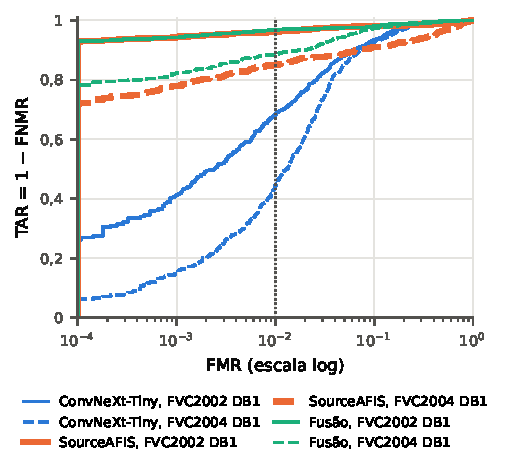
\includegraphics[width=0.64\columnwidth]{figures/roc.pdf}
\caption{Curvas ROC da ConvNeXt-Tiny, do SourceAFIS e da fusão nos 30 dedos de teste das duas bases, todos os pares, seed 2026. A linha pontilhada marca FMR de 1\%.}
\label{fig:roc}
\end{figure}

\begin{figure}[t]
\centering
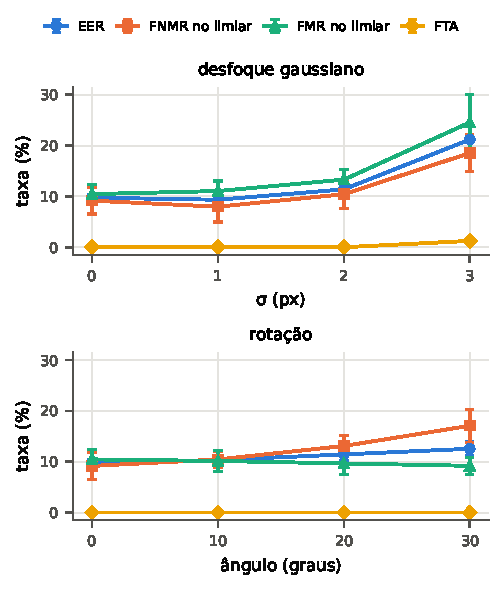
\includegraphics[width=0.7\columnwidth]{figures/robustness.pdf}
\caption{Robustez da ConvNeXt-Tiny nos 30 dedos de teste da FVC2002 DB1 com o limiar congelado: desfoque (acima) e rotação (abaixo), média $\pm$ desvio de três seeds.}
\label{fig:robustez}
\end{figure}

No Experimento~C, a EER da ConvNeXt-Tiny vai de 3,84\% na validação para 7,87\% no teste da FVC2002 DB1 e para 8,32\% e 10,42\% na FVC2004 DB1: a queda maior está entre a validação e o teste da própria base. No limiar congelado, a FNMR sobe de 3,93\% na validação para 9,56\%, 10,79\% e 14,10\% (Fig.~\ref{fig:dist}), e a TAR a FAR de 1\% cai de 68,8\% na FVC2002 DB1 para 46,5\% e 50,9\% na FVC2004 DB1.

\emph{Referências.} Sem ajuste fino, a ConvNeXt-Tiny tem EER de 29,49\%, 34,88\% e 34,75\% nas três avaliações de teste; o ajuste reduz a EER em 21,6 (18,5 a 24,9), 26,6 (22,9 a 29,5) e 24,3 pontos (21,2 a 27,3). O SourceAFIS tem EER de 2,71\% na FVC2002 DB1, 5,16 pontos abaixo da ConvNeXt-Tiny (3,4 a 7,0). Na FVC2004 DB1 ele tem 9,31\% e 12,18\%, 0,98 ($-2{,}1$ a 3,9) e 1,75 ponto ($-0{,}1$ a 3,9) acima da ConvNeXt-Tiny, e os dois intervalos contêm zero. Mesmo com EER parecida, os erros se distribuem de outro modo: no limiar da validação, o SourceAFIS tem FMR de 2,02\% e FNMR de 12,62\% nos dedos de teste da FVC2004 DB1, e sua TAR a FAR de 1\% é 85,0\%, contra 46,5\% da CNN. A fusão, com $w$ de 0,6 ou 0,7 conforme a seed, tem EER de $2{,}73\pm0{,}11$\%, $4{,}96\pm0{,}25$\% e $6{,}86\pm0{,}41$\% (Fig.~\ref{fig:roc}). Na FVC2002 DB1 a diferença para o SourceAFIS é de 0,02 ponto ($-0{,}7$ a 0,8). Na FVC2004 DB1 ela fica 4,35 (2,3 a 6,7) e 5,32 pontos (4,1 a 6,9) abaixo do SourceAFIS e 3,37 (2,3 a 4,8) e 3,57 pontos (2,6 a 4,6) abaixo da CNN sozinha.

\begin{figure*}[t]
\centering
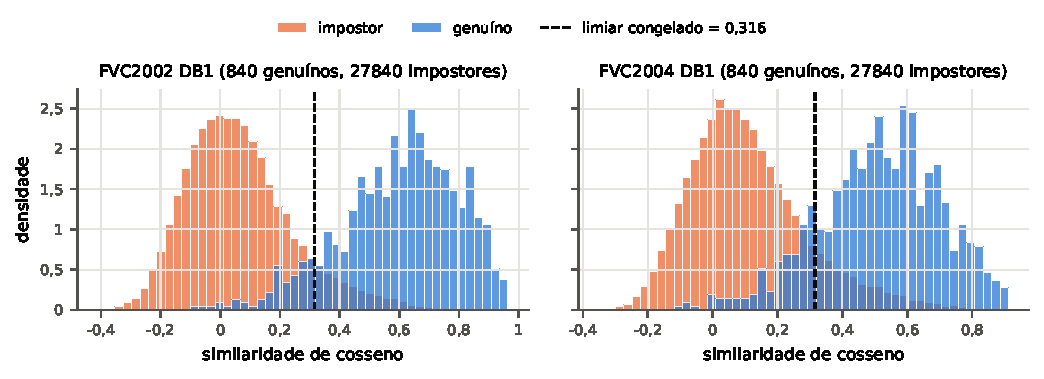
\includegraphics[width=0.66\textwidth]{figures/distributions.pdf}
\caption{Scores genuínos e impostores da ConvNeXt-Tiny (seed 2026) nos 30 dedos de teste de cada base, todos os pares, com o limiar congelado dessa seed (0,380).}
\label{fig:dist}
\end{figure*}

\begin{figure*}[t]
\centering
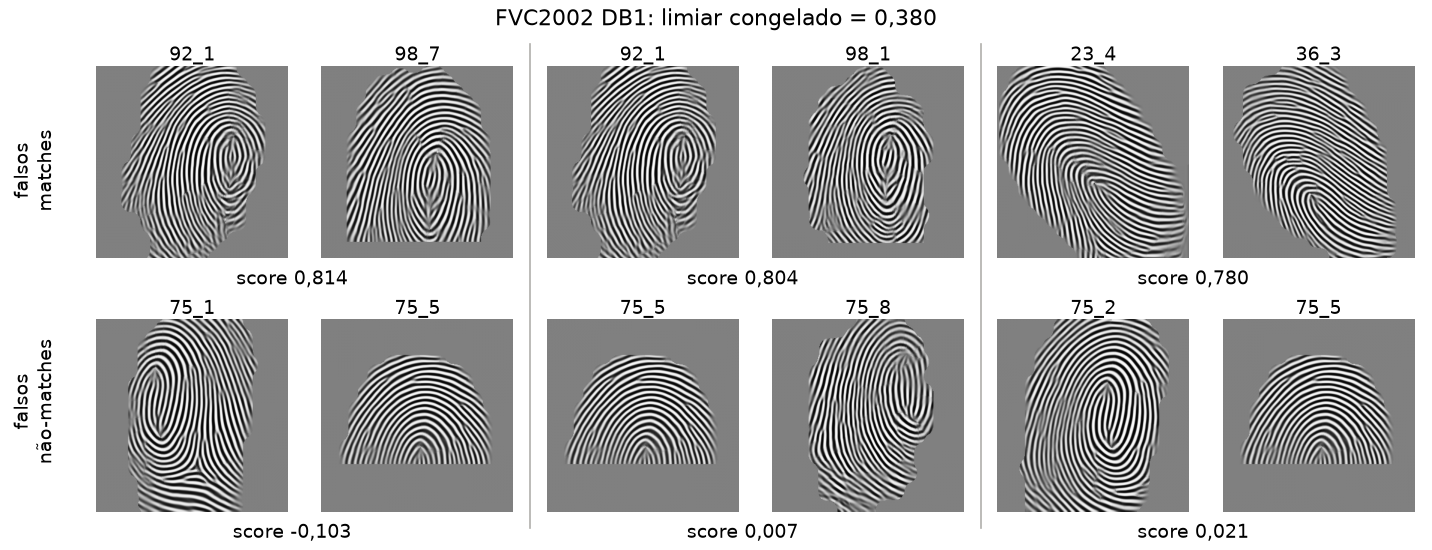
\includegraphics[width=0.66\textwidth]{figures/errors_fvc2002_db1.png}\\[2pt]
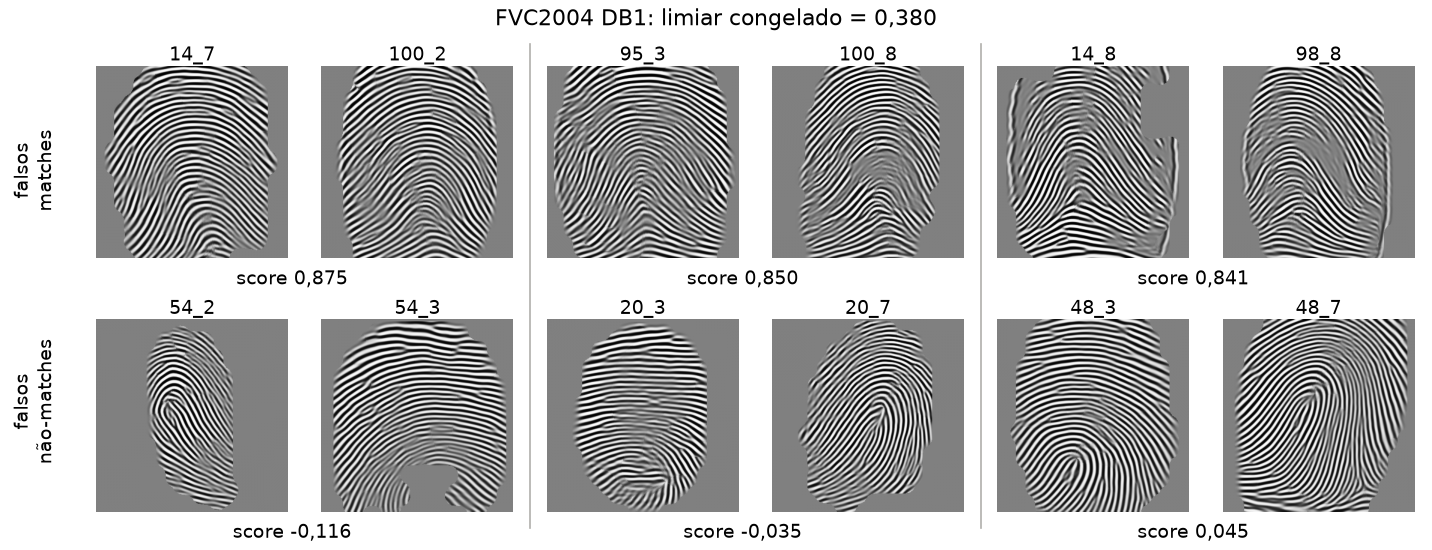
\includegraphics[width=0.66\textwidth]{figures/errors_fvc2004_db1.png}
\caption{Três falsos matches (linha de cima) e três falsos não-matches (linha de baixo) da ConvNeXt-Tiny na FVC2002 DB1 (acima) e na FVC2004 DB1 (abaixo), seed 2026, limiar 0,380. Cada par mostra as duas amostras como a rede as recebe (janela 320$\times$320 com realce), com o score do par.}
\label{fig:erros}
\end{figure*}

\subsection{Experimento D e ablação}

\begin{table}[t]
\centering
\caption{Experimento D: ConvNeXt-Tiny nos 30 dedos de teste da FVC2002 DB1, limiar congelado. Média $\pm$ desvio-padrão de três seeds (AUC: só a média). Taxas em \%.}
\label{tab:robustez}
\footnotesize
\setlength{\tabcolsep}{2.5pt}
\begin{tabular}{@{}lccccc@{}}
\toprule
Nível & EER & AUC & FMR & FNMR & FTA \\
\midrule
Original & $7{,}87\pm0{,}29$ & 0,976 & $6{,}39\pm1{,}02$ & $9{,}56\pm1{,}34$ & 0,00 \\
\midrule
Desfoque $\sigma=1$ & $7{,}93\pm0{,}42$ & 0,977 & $6{,}81\pm1{,}18$ & $9{,}01\pm1{,}96$ & 0,00 \\
Desfoque $\sigma=2$ & $17{,}95\pm0{,}67$ & 0,903 & $13{,}80\pm3{,}71$ & $21{,}27\pm2{,}24$ & 0,00 \\
Desfoque $\sigma=3$ & $27{,}25\pm1{,}77$ & 0,800 & $75{,}73\pm7{,}66$ & $5{,}52\pm2{,}45$ & 1,25 \\
\midrule
Rotação $10^\circ$ & $8{,}13\pm0{,}18$ & 0,973 & $6{,}07\pm1{,}10$ & $10{,}91\pm1{,}61$ & 0,00 \\
Rotação $20^\circ$ & $9{,}32\pm0{,}47$ & 0,967 & $5{,}97\pm1{,}39$ & $14{,}40\pm1{,}65$ & 0,00 \\
Rotação $30^\circ$ & $10{,}67\pm0{,}55$ & 0,958 & $5{,}84\pm1{,}60$ & $18{,}45\pm3{,}33$ & 0,00 \\
\bottomrule
\end{tabular}
\end{table}

A Tabela~\ref{tab:robustez} e a Fig.~\ref{fig:robustez} trazem os quatro níveis de cada degradação. O desfoque com $\sigma=1$ pixel não muda a EER; esse nível está dentro da faixa do aumento de dados do treino ($\sigma$ até 1,5). Com $\sigma=2$, a EER vai a 17,95\% e a FNMR a 21,27\%. Com $\sigma=3$, a EER chega a 27,25\%, a FMR a 75,73\% e a FNMR cai para 5,52\%, com 3 das 240 imagens marcadas como FTA. A rotação quase não muda a FMR, que fica entre 5,8\% e 6,1\%, e leva a FNMR a 18,45\% a $30^\circ$. Na ablação, a ConvNeXt-Tiny sem realce tem EER de $6{,}89\pm0{,}78$\% na FVC2002 DB1; a diferença para a versão com realce é de $-0{,}97$ ponto ($-2{,}8$ a 0,7). Na FVC2004 DB1 o realce ajuda: sem ele, a EER é $10{,}35\pm0{,}72$\% nos dedos de teste, 2,03 pontos acima (0,3 a 3,4), e $11{,}29\pm0{,}84$\% no protocolo oficial, 0,86 ponto acima ($-0{,}6$ a 2,3).

\subsection{Configuração base e configuração otimizada}

Depois de fechados os resultados acima, tentamos reduzir a FMR e a FNMR só da ConvNeXt-Tiny, em duas etapas. Cada uma das dezesseis tentativas concluídas foi aceita ou descartada pela EER de validação, e a lista completa está em \texttt{otimizacao/README.md}. Na primeira etapa, o treino recebe as bases DB2, DB3 e DB4 da FVC2002, de outros sensores e voluntários (390 dedos, 40 épocas), e o sistema soma os scores de duas ConvNeXt-Tiny, uma com realce de Gabor e outra só com a normalização de Hong. Na segunda, entram também as bases DB2, DB3 e DB4 da FVC2004 e a U.are.U da Neurotechnology~\cite{neurotech2026uareu}, 785 dedos ao todo. Quarenta deles, 20 da FVC2004 DB2 e 20 da DB3, saem do treino e vão para a validação, o que deixa 745 no treino. Decidimos ampliar a validação depois de examinar os erros de uma execução na FVC2004 DB1, que continua fora do treino. O sistema soma quatro ConvNeXt-Tiny por seed, e cada score é normalizado contra os 100 dedos de treino mais próximos de cada imagem.

\begin{table}[t]
\centering
\caption{ConvNeXt-Tiny: configuração base e tentativas de otimização. Média de três seeds, taxas em \%, FMR e FNMR no limiar congelado de cada configuração. As duas últimas linhas usam score normalizado, e a última soma as redes das três seeds num só sistema.}
\label{tab:otim}
\footnotesize
\setlength{\tabcolsep}{2.5pt}
\begin{tabular}{@{}lcccccc@{}}
\toprule
 & \multicolumn{3}{c}{FVC2002 DB1, teste} & \multicolumn{3}{c}{FVC2004 DB1-A, oficial} \\
Configuração & EER & FMR & FNMR & EER & FMR & FNMR \\
\midrule
Base (60 dedos, Gabor) & 7,87 & 6,39 & 9,56 & 10,42 & 7,57 & 14,10 \\
390 dedos, Gabor + Hong & 4,05 & 3,56 & 4,56 & 6,23 & 3,52 & 10,95 \\
745 dedos, 4 redes & 3,07 & 3,15 & 3,06 & 4,30 & 2,25 & 8,05 \\
745 dedos, 12 redes & 2,74 & 2,75 & 2,74 & 3,82 & 1,88 & 7,50 \\
\bottomrule
\end{tabular}
\end{table}

A Tabela~\ref{tab:otim} compara as configurações. Com as duas mudanças da primeira etapa, a EER cai 3,8 pontos na FVC2002 DB1 (IC de 95\% de 2,3 a 5,3) e 4,2 no protocolo oficial (3,2 a 5,2). Na segunda etapa, a soma das doze redes chega a EER de 2,74\% na FVC2002 DB1, 3,33\% nos 30 dedos de teste da FVC2004 DB1 e 3,82\% no protocolo oficial, quedas de 5,1 (3,5 a 7,0), 5,0 (3,5 a 6,9) e 6,6 pontos (5,4 a 7,8) sobre a base. Esses intervalos, com \num{2000} reamostragens, valem para os sistemas treinados e os dedos avaliados, e não medem a variação entre novos treinos. As bases DB2 a DB4 da FVC2004 seguem o mesmo roteiro de coleta da DB1, então a segunda etapa mede a troca de sensor e de voluntários, e não mais a troca de tipo de coleta. Seis dos doze treinos rodaram numa GPU A100, e os demais na RTX~4060. O conjunto de 12 redes leva cerca de 110~ms por imagem na GPU e ocupa 1,3~GB. Os demais resultados deste artigo usam a configuração base, que segue a regra de treinar só na FVC2002 DB1.

% ---------------------------------------------------------------------------
\section{Análise e discussão}
\label{sec:discussao}

\subsection{Transferência do limiar}

O limiar fixado na validação se transfere de forma imperfeita, e a perda maior ocorre dentro da própria base: a EER dobra entre os 20 dedos de validação e os 30 de teste da FVC2002 DB1, e a FNMR no limiar passa de 3,9\% para 9,6\%. A validação escolhe a época e o limiar nos mesmos pares, o que a torna otimista, e 20 dedos dão uma estimativa ruidosa. O SourceAFIS, que usa a validação só para o limiar, quase não muda entre validação e teste (2,61\% e 2,71\%). Entre os dois testes de 30 dedos, a EER da CNN passa de 7,87\% para 8,32\%, e é o SourceAFIS que mais piora, de 2,71\% para 9,31\%. O erro dominante da CNN na FVC2004 DB1 é de rejeição, com FNMR de 10,8\% e 14,1\% no limiar. As imagens brutas da FVC2004 DB1 são menos nítidas (variância do Laplaciano de 635 em média, contra \num{1643}), e a coleta pediu distorções de propósito; não isolamos nenhum dos dois efeitos.

\subsection{Realce, minúcias e fusão}

Na fase anterior do projeto, em que o treino reunia bases de outros sensores e a validação vinha de sensores não vistos, o realce reduziu a EER de validação da ResNet-50 de 8,06\% para 6,54\% (\texttt{results/fase\_anterior/tuning\_lso.csv}). Aqui ele não ajuda na base do treino e reduz a EER em 2 pontos nos 30 dedos de teste da FVC2004 DB1; no protocolo oficial a redução é de 0,9 ponto e o intervalo contém zero. Nossa hipótese, não testada de outra forma, é que o realce apaga a aparência do sensor: quando treino e teste vêm do mesmo sensor, ela não atrapalha, e a normalização de Hong preserva detalhes que o realce remove. O realce também é a etapa mais cara do sistema: acrescenta de 50 a 100~ms por imagem em CPU, várias vezes os 9~ms da rede na GPU.

O comparador de minúcias continua muito à frente na FVC2002 DB1, mas perde mais que a CNN na troca de sensor. O ganho da fusão sugere que os erros dos dois são em parte complementares, embora não tenhamos medido a sobreposição: ela iguala o SourceAFIS na primeira base e fica 4,4 e 5,3 pontos abaixo dele na segunda. Os modelos de tamanho fixo que se aproximam dos comparadores de minúcias nas bases FVC usaram centenas de milhares de imagens~\cite{engelsma2021deepprint,grosz2024afrnet}; o DeepPrint tem TAR de 97,5\% a FAR de 0,1\% na FVC2004 DB1-A, e a ConvNeXt-Tiny tem 50,9\% a FAR de 1\% no mesmo protocolo.

\subsection{Comparação das CNNs e custo}

Na base do treino as três redes empatam dentro dos intervalos. A diferença aparece na troca de sensor: a ConvNeXt-Tiny fica de 3,7 a 4,9 pontos abaixo das outras duas, com intervalos que excluem zero, e a FNMR da ResNet-50 e da EfficientNet-B0 na FVC2004 DB1 passa de 19\%, contra 10,8\% da ConvNeXt-Tiny. A ConvNeXt-Tiny usa convoluções de $7\times7$ e LayerNorm no lugar da BatchNorm~\cite{liu2022convnext}; não isolamos qual dessas diferenças explica o resultado. As três redes usam a configuração da fase anterior, ajustada com a ResNet-50 e a ConvNeXt-Tiny, o que pode desfavorecer a EfficientNet-B0. Nesta GPU ela é a mais lenta com lote 1, apesar de ter 6,5 vezes menos parâmetros; sua vantagem são os 17,6~MB de pesos.

\subsection{Robustez}

Sob desfoque forte o erro passa a ser de segurança: com $\sigma=3$ nas duas imagens, o sistema aceita 76\% dos impostores. Nossa hipótese para $\sigma=3$ é que o realce produz cristas a partir de uma imagem sem detalhe, as impressões ficam parecidas para a rede e os scores impostores passam do limiar; não repetimos o teste com a rede sem realce para confirmá-la. O controle de qualidade mede só a área da ROI, que o desfoque quase não muda, e marcou 3 das 240 imagens. Seria preciso um critério de nitidez, como um limiar na variância do Laplaciano fixado na validação. A rotação eleva só a FNMR. O treino usou rotações de até $30^\circ$, mas no teste cada imagem recebe um sinal sorteado, e a rotação relativa de um par chega a $60^\circ$.

\subsection{Análise de erros}

A Fig.~\ref{fig:erros} mostra os três falsos matches de maior score e os três falsos não-matches de menor score da ConvNeXt-Tiny em cada base.

\emph{FVC2002 DB1.} Os falsos matches têm scores de 0,78 a 0,81, bem acima do limiar de 0,380. Dois deles juntam a impressão 92\_1 a duas impressões do dedo 98 (98\_7 e 98\_1), laços com o núcleo no centro da janela e fluxo de cristas parecido; o terceiro, 23\_4 com 36\_3, junta dois laços com a mesma inclinação. Hipótese: o embedding codifica a classe do padrão e o fluxo global, e pouco do detalhe que separa dedos da mesma classe. Os três falsos não-matches envolvem a mesma impressão, 75\_5, que tem 99~mm$^2$ de área, contra 144 a 197~mm$^2$ das outras impressões do dedo. Ela mostra só a ponta do dedo, sem o núcleo, e os pares ficam sem região comum suficiente (scores de $-0{,}10$ a 0,02). A figura mostra só os casos extremos, e a repetição da mesma impressão nesses extremos não diz como se distribuem os demais falsos não-matches.

\emph{FVC2004 DB1.} Os falsos matches têm scores ainda maiores, de 0,84 a 0,88, em pares com cristas quase horizontais no centro da janela, e dois envolvem imagens de nitidez abaixo da média da base. Os falsos não-matches são uma faixa estreita de 94~mm$^2$, um par em que o realce produz padrões diferentes para o mesmo dedo e um par que mostra regiões diferentes do dedo. Hipótese: em capturas de pouco contraste ou parciais, o realce com período único por imagem gera um padrão regular que o embedding não distingue bem, e a falta de alinhamento por pose deixa pares do mesmo dedo sem região comum.

\subsection{Limitações}

A configuração de treino (realce de Gabor, 80 épocas e taxa de aprendizado) veio de uma fase anterior do projeto, quando só o conjunto B estava disponível e seus 10 dedos de cada base eram o teste. Esses dedos estão entre as 110 identidades divididas aqui: a seed 42 pôs sete no treino, um na validação e dois, 107 e 109, no teste das duas bases. As escolhas daquela fase se basearam em parte em resultados de teste que incluíam esses dois dedos; nenhuma escolha posterior usou o teste. Sem os pares que envolvem 107 ou 109 (restam 784 genuínos e \num{24192} impostores), a EER da ConvNeXt-Tiny é 7,95\% na FVC2002 DB1 e 7,94\% na FVC2004 DB1, a da ResNet-50 é 9,42\% e 12,93\% e a da EfficientNet-B0 é 7,82\% e 11,77\%; na FVC2002 DB1 a EfficientNet-B0 passa à frente da ConvNeXt-Tiny por 0,13 ponto, dentro dos intervalos, e na FVC2004 DB1 a ordem não muda (\texttt{results/sensitivity\_setb.csv}). O treino usa 60 dedos de um único sensor. A ResNet-50 e a EfficientNet-B0 não tiveram ajuste próprio de hiperparâmetros. O SourceAFIS usou os parâmetros padrão, e não comparamos sua latência com a da CNN. O desfoque e a rotação atingem as duas imagens do par e foram medidos só na FVC2002 DB1. O Experimento~B é parcial: não tem a CNN de uma segunda equipe.

% ---------------------------------------------------------------------------
\section{Conclusão}
\label{sec:conclusao}

Uma ConvNeXt-Tiny ajustada com ArcFace em 480 imagens de 60 dedos da FVC2002 DB1 chega a 7,87\% de EER nos dedos de teste da mesma base e, sem novo ajuste, a 8,32\% e 10,42\% na FVC2004 DB1, que ficou fora do ajuste. Na base do treino ela empata com a ResNet-50 e a EfficientNet-B0; na troca de sensor fica de 3,7 a 4,9 pontos abaixo delas. Um comparador de minúcias ainda ganha com folga na FVC2002 DB1, mas perde mais na troca de sensor, e a fusão dos dois scores tem a menor EER da configuração base na FVC2004 DB1 (4,96\% e 6,86\%). A validação com 20 dedos estima metade da EER de teste, e o desfoque forte faz o sistema aceitar 76\% dos impostores sem que o controle por área perceba. Com mais bases no treino e a soma de várias ConvNeXt-Tiny, a EER da rede cai para 2,74\% e 3,82\% (Tabela~\ref{tab:otim}).

Os próximos passos são alinhar as impressões pela pose antes do recorte, estimar o período de crista por região e acrescentar um critério de nitidez ao controle de qualidade. Código, protocolos e scores estão em \repourl, versão \texttt{\repoversion}.

\bibliographystyle{IEEEtran}
\bibliography{IEEEabrv,refs}

\end{document}
